\documentclass[11pt,a4paper]{article}

\usepackage[margin=2cm]{geometry}
\usepackage{amsmath}
\usepackage{amssymb}
\usepackage{booktabs}
\usepackage{graphicx}
\usepackage[colorlinks=true,linkcolor=blue,citecolor=blue,urlcolor=blue]{hyperref}

\title{Benchmarking a Basic Triple-Loop Matrix Multiplication\\
in Python, Java, C and Go}
\author{Aythami Lorenzo}
\date{October 2026 --- Individual Assignment 1, Big Data}

\begin{document}

\maketitle

\begin{abstract}
We study the behavior of several basic matrix multiplication algorithms used for
multiplying dense square matrices in four programming languages: Python, Java, C
and Go. All implementations execute the same naive \(i\text{-}j\text{-}k\) triple
loop over \texttt{float64} values with row-major storage, so the four
implementations differ only in language and runtime. We perform an analysis of
the following elements: kernel-only runtime per multiplication (median and
interquartile range over 7 repetitions after 3 warm-ups), peak resident set
size of the process, and result checksums validated against a NumPy
reference. Our experiments provide a reproducible benchmark of \(O(n^3)\)
algorithms across a variety of input sizes (\(n = 10\) to \(1000\) elements per
side) to guide future research in the cost of language runtimes for naive
numeric kernels. Based on our experiments, we recommend C when raw throughput is
the goal, Go as a portable near-C alternative with a simple memory profile,
Java once its just-in-time warm-up is accounted for, and Python only for small
matrices or prototyping, where its 50--90$\times$ slowdown remains affordable.
\end{abstract}

\tableofcontents

\section{Introduction and objective}

Dense matrix multiplication is the canonical workload for studying how a
programming language and its runtime affect the cost of a purely arithmetic
\(O(n^3)\) kernel. Because the algorithm and its memory-access pattern---a
naive triple loop with a strided column scan---are identical across
implementations, any observed difference in runtime or memory can be attributed
to the language, its compiler or just-in-time (JIT) engine, and its runtime
system.

The objective of this assignment is to answer the research question:
\emph{how does the matrix size \(n\) affect the runtime and the peak memory of
a basic \(O(n^3)\) triple-loop multiplication across four implementations?} The
assignment requires Python, Java and C; we add Go as a clearly labelled fourth
implementation that follows the identical algorithm and protocol, so it is
compared but never substitutes the required three-language comparison.

\section{Background}

The textbook algorithm computes each entry of \(C = A B\) as a dot product of
one row of \(A\) with one column of \(B\), giving \(n^3\) multiply--accumulate
operations, i.e.\ \(\Theta(n^3)\) arithmetic work~\cite{knuth1997}. Gauss
already observed that the operation count can be reduced
asymptotically~\cite{strassen1969}, but the basic triple loop remains the
reference for clarity and the subject of this study.

Arithmetic is only part of the cost: the inner loop streams one row of \(A\)
sequentially while jumping through \(B\) with a stride of \(8n\) bytes, so once
the working set (three matrices, \(24n^2\) bytes) exceeds the last-level cache,
each iteration becomes a memory transaction~\cite{hennessy2017,frigo1999}. All
values are IEEE-754 \texttt{float64} numbers~\cite{ieee754}, so results are
deterministic for a fixed evaluation order and comparable across languages up
to the last unit in the last place (ulp).

\section{Methodology}

\subsection{Implementations and protocol}

All four kernels perform the same loop nest (\(i\), then \(j\), then \(k\))
writing into a pre-allocated \texttt{float64} row-major output buffer; no
library call (BLAS, \texttt{numpy.matmul}, \dots) executes inside the measured
kernel. NumPy is used only to generate the shared inputs~\cite{harris2020} and
to compute the correctness reference; the measured Python kernel uses plain
lists of lists of \texttt{float}.

\begin{itemize}
  \item \textbf{Shared inputs.} Every language loads the same
  \texttt{matrixA\_n.bin} / \texttt{matrixB\_n.bin} files (little-endian
  \texttt{float64}, row-major), generated once with seed 42; generation and
  loading happen outside the timed region.
  \item \textbf{Timing boundary.} The timer surrounds only the triple loop; a
  sequential row-major checksum is computed afterwards so the compiler cannot
  eliminate the work. Only monotonic clocks: \texttt{System.nanoTime()} (Java),
  \texttt{clock\_gettime(CLOCK\_MONOTONIC)} (C), \texttt{time.Now()} (Go),
  \texttt{time.perf\_counter\_ns()} (Python).
  \item \textbf{Warm-up and repetitions.} Three warm-up runs (recorded,
  excluded) plus seven measured repetitions; we report the median and the
  interquartile range (IQR). Multiplications shorter than \(\approx\)2\,ms run
  as a batch of \(K\) multiplications inside the timed region, reporting time
  per multiplication (\(K\) stored in the CSV).
  \item \textbf{Budgets and sizes.} 60\,s per multiplication,
  \(\approx\)2\,GB memory; a budget overrun is a result (exit code 3), never an
  invented time. Sizes: \(n \in \{10, 25, 50, 100, 200, 500, 1000\}\).
  \item \textbf{Memory metric.} Peak resident set size (peak RSS) read from the
  kernel watermark \texttt{/proc/self/status} (\texttt{VmHWM}) in \emph{all
  four} languages---one metric, one counter, one tool. The theoretical array
  storage \(24n^2\) and, for Java, the peak heap are reported separately and
  never compared as if identical.
  \item \textbf{Correctness.} Before any benchmark, each implementation is
  validated against a NumPy \texttt{float64} reference with
  \texttt{rtol}=1e-9, \texttt{atol}=1e-12 on identity, zero, known-answer
  \(3\times3\) and random small matrices. On the campaign inputs the four
  checksums agree exactly for \(n \le 500\) and within 1 ulp at \(n = 1000\).
\end{itemize}

\begin{table}[t]
\centering
\caption{Execution environment of the campaign (WSL2 on the student's
machine).}
\label{tab:env}
\footnotesize
\begin{tabular}{@{}ll@{}}
\toprule
Component & Value \\
\midrule
CPU & Intel Core i7-10750H @ 2.6\,GHz (6 cores / 12 threads) \\
Host memory / OS & 16\,GB DDR4, Windows 11 host \\
Execution OS & WSL2, Ubuntu 26.04 LTS, kernel 6.18.33.2 \\
VM memory / CPUs & \(\approx\)7.7\,GB RAM, 12 logical processors \\
C compiler & gcc 15.2.0, \texttt{-O2 -std=c11 -Wall -Wextra} \\
Java & OpenJDK 17.0.20.1, Maven 3.9.12 \\
Go / Python & Go 1.27.2 / Python 3.14.4 (numpy, pandas, matplotlib) \\
\bottomrule
\end{tabular}
\end{table}

All builds, tests, benchmarks and plots ran inside WSL2 on the student's
machine (Table~\ref{tab:env}); native Windows binaries are blocked by Smart App
Control on this computer, so only measurements taken in this environment are
reported. Each configuration ran sequentially, once, on an otherwise idle
machine.

\section{Results}

\subsection{Runtime}

Table~\ref{tab:median} reports the median time per multiplication with the IQR
of the seven measured repetitions; Figure~\ref{fig:median} shows the same data
on log--log axes with the \(O(n^3)\) reference slope.

\begin{table}[t]
\centering
\caption{Median time per multiplication in ms (IQR in parentheses), 7
repetitions after 3 warm-ups. ``--'': budget exceeded, no measurement.}
\label{tab:median}
\footnotesize
\begin{tabular}{@{}rcccc@{}}
\toprule
\(n\) & C & Go & Java & Python \\
\midrule
10    & 0.00086 (0.00003) & 0.0027 (0.00011) & 0.058 (0.016)   & 0.078 (0.003) \\
25    & 0.016 (0.0003)    & 0.056 (0.002)    & 0.16 (0.030)    & 1.12 (0.043) \\
50    & 0.158 (0.012)     & 0.421 (0.010)    & 1.26 (0.14)     & 8.73 (0.11) \\
100   & 1.47 (0.04)       & 3.31 (0.11)      & 1.95 (0.16)     & 75.3 (4.8) \\
200   & 13.8 (0.3)        & 25.6 (0.5)       & 17.0 (0.6)      & 672 (6.2) \\
500   & 238 (1.7)         & 405 (13)         & 350 (7.6)       & 13\,711 (146) \\
1000  & 5\,672 (88)       & 6\,414 (58)      & 17\,539 (68)    & -- \\
\bottomrule
\end{tabular}
\end{table}

\begin{figure}[t]
\centering
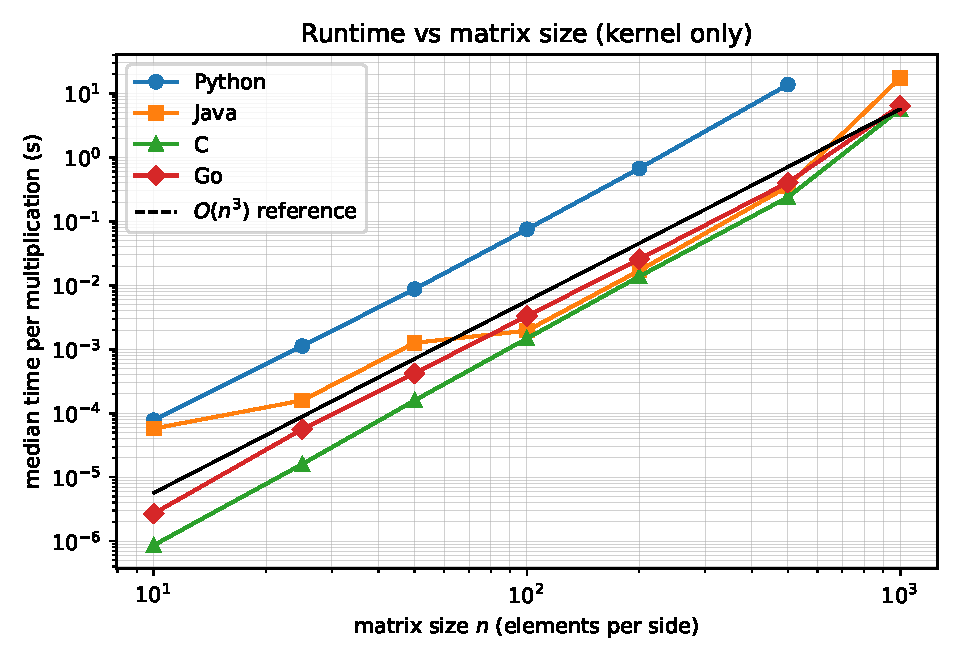
\includegraphics[width=0.72\linewidth]{figures/median_time_vs_size.pdf}
\caption{Median kernel runtime vs matrix size (log--log) with the
\(O(n^3)\) reference slope. Python has no point at \(n=1000\): the run exceeded
the 60\,s budget.}
\label{fig:median}
\end{figure}

\begin{figure}[t]
\centering
\begin{minipage}[t]{0.49\linewidth}
\centering
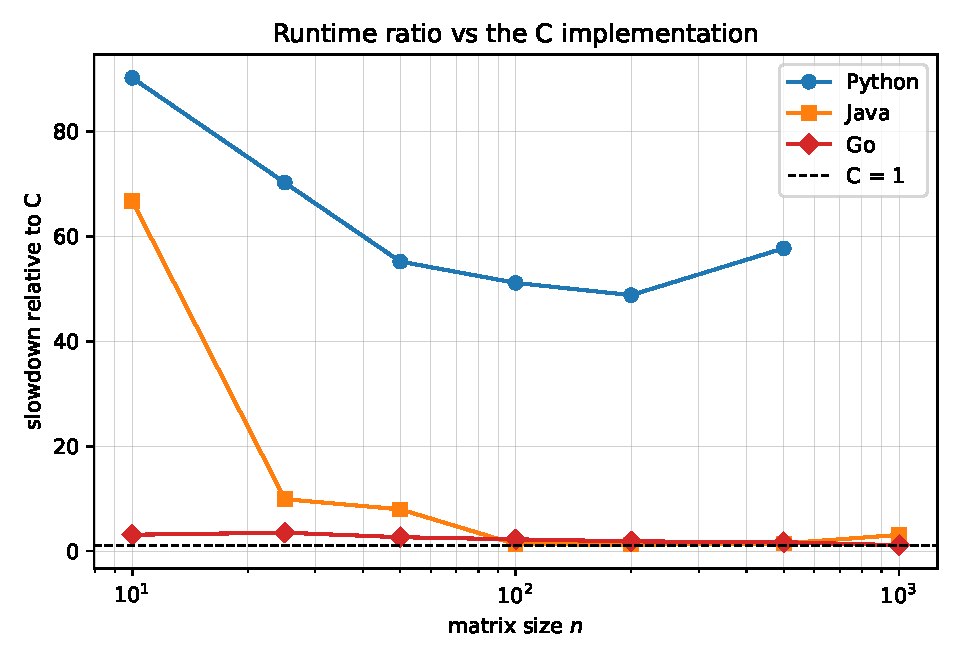
\includegraphics[width=\linewidth]{figures/slowdown_vs_c.pdf}
\end{minipage}\hfill
\begin{minipage}[t]{0.49\linewidth}
\centering
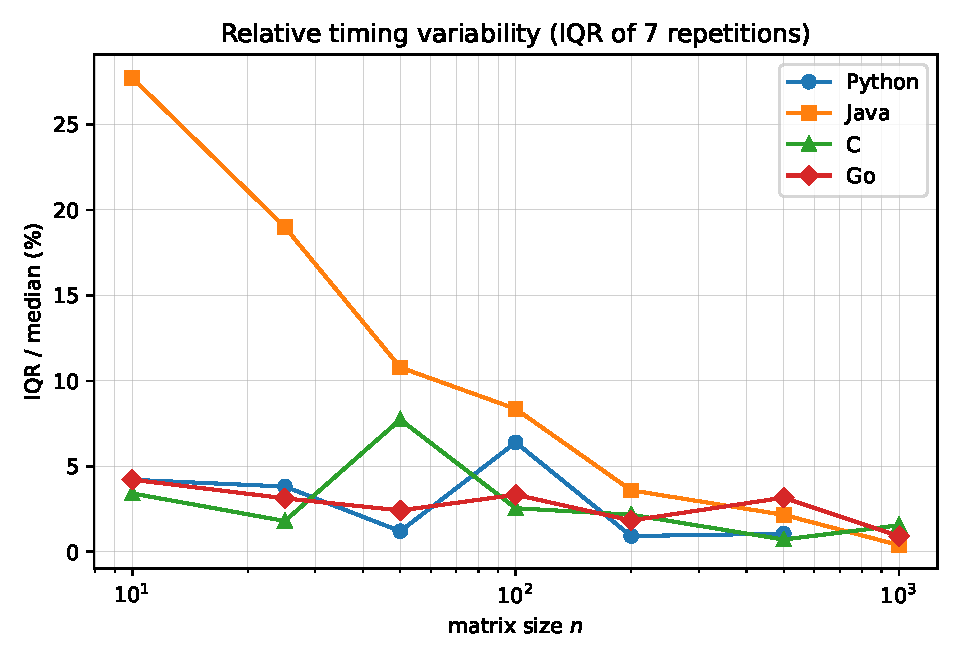
\includegraphics[width=\linewidth]{figures/timing_variability.pdf}
\end{minipage}
\caption{(Left) Runtime ratio of each language relative to C. (Right) Relative
timing variability (IQR/median over the 7 measured repetitions).}
\label{fig:ratios}
\end{figure}

Figure~\ref{fig:ratios} (left) shows the slowdown relative to C: C is fastest
at every size; Go runs 1.1--3.5$\times$ slower, Python 50--90$\times$ slower,
and Java moves from 67$\times$ slower at \(n=10\) to 1.2--1.5$\times$ in the
mid range and 3.1$\times$ at \(n=1000\). All curves follow the \(O(n^3)\) trend
over three orders of magnitude, with a steeper segment between \(n=500\) and
\(n=1000\) discussed in Section~\ref{sec:discussion}. Right:
Figure~\ref{fig:ratios} (right) reports the IQR as a percentage of the median:
C, Go and Python stay mostly below 5\,\% once the timed region is long enough,
while Java shows 8--28\,\% variability for \(n \le 100\)---consistent with JIT
compilation still progressing during the measurement window---and drops below
4\,\% for \(n \ge 200\).

\subsection{Memory}

\begin{table}[t]
\centering
\caption{Peak RSS in MB (from \texttt{VmHWM}) and theoretical array storage
\(24n^2\). ``--'': not recorded (budget exceeded).}
\label{tab:memory}
\footnotesize
\begin{tabular}{@{}rrcccc@{}}
\toprule
\(n\) & \(24n^2\) & C & Go & Java & Python \\
\midrule
10   & 0.0  & 2.1  & 2.6  & 46.2  & 16.9 \\
50   & 0.1  & 2.1  & 2.8  & 46.4  & 17.2 \\
100  & 0.2  & 2.3  & 3.0  & 46.9  & 18.0 \\
200  & 1.0  & 3.0  & 4.3  & 48.4  & 21.8 \\
500  & 6.0  & 8.1  & 13.3 & 59.0  & 48.7 \\
1000 & 24.0 & 26.1 & 35.5 & 117.4 & -- \\
\bottomrule
\end{tabular}
\end{table}

\begin{figure}[t]
\centering
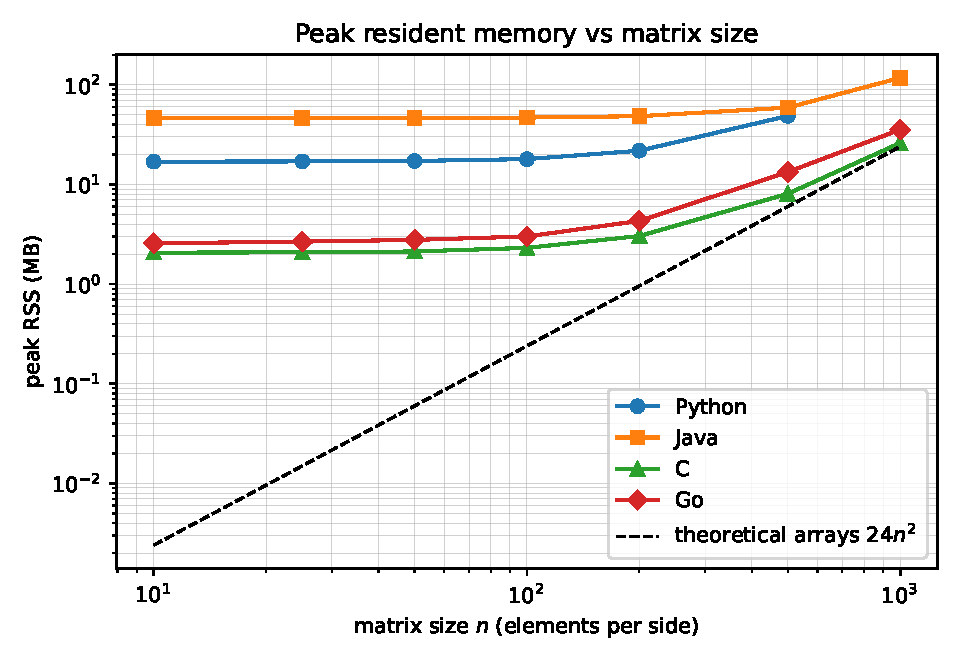
\includegraphics[width=0.72\linewidth]{figures/peak_rss_vs_size.pdf}
\caption{Peak resident set size vs matrix size, with the theoretical array
storage \(24n^2\) as reference.}
\label{fig:peak}
\end{figure}

Table~\ref{tab:memory} and Figure~\ref{fig:peak} show two regimes: a flat
runtime floor at small \(n\) (C: 2.1\,MB; Go: 2.6\,MB; Python: 16.9\,MB; JVM:
46.2\,MB) dominated by the interpreter, loader and runtime structures, and a
growth regime where the \(24n^2\) bytes of matrix data dominate. At
\(n=1000\), C peaks at 26.1\,MB---the theoretical 24\,MB plus
\(\approx\)2\,MB of process overhead---while the JVM peaks at 117.4\,MB, of
which only \(\approx\)3\,MB is heap.

\section{Discussion}
\label{sec:discussion}

\textbf{Complexity and the cache cliff.} The measured curves track the
theoretical \(O(n^3)\) law over three orders of magnitude, but the growth from
\(n=500\) to \(n=1000\) is steeper than the pure arithmetic prediction
(\(\times 8\)): \(\times 23.9\) for C, \(\times 15.8\) for Go and
\(\times 50.1\) for Java. The cause is the memory hierarchy: at \(n=1000\) the
three matrices occupy 24\,MB, well above the 12\,MB last-level cache of the
i7-10750H, so the strided column reads of \(B\) become cache
misses~\cite{frigo1999,hennessy2017}. This is a property of the algorithm and
the machine, not of any language.

\textbf{Language effects.} C is fastest at all sizes. Go stays within
1.1--3.5$\times$ of C---its ahead-of-time compiled kernel runs without a
garbage collector inside the loop---at the price of a slightly higher RSS
(35.5\,MB vs 26.1\,MB at \(n=1000\)). Java converges toward C in the mid range
once the JIT compiles the hot loop, then loses ground again at \(n=1000\); its
higher small-size variability reflects the same warm-up effect. Python is
50--90$\times$ slower throughout; its flat interpreter overhead also dominates
at small \(n\), where the reported times are those of an interpreter loop
rather than of arithmetic.

\textbf{Budget outcome.} Python at \(n=1000\) required 178.6\,s for a single
probe multiplication, exceeding the 60\,s budget; the runner exited with code 3
and recorded no time or memory row for that configuration. The largest
completed size therefore differs per language (Python: \(n=500\); the other
three: \(n=1000\)), which is itself a protocol result and is reported as such.

\section{Conclusions}

The basic i-j-k triple-loop multiplication behaves as \(O(n^3)\) predicts up to
the point where the working set leaves the last-level cache, at which point
memory traffic steepens the curve for every language alike. Language choice
changes the constant factor, not the complexity: C is fastest; Go provides
near-C speed with a clean, portable build; Java is competitive after JIT
warm-up but needs it accounted for; Python is one to two orders of magnitude
slower and hits the 60\,s budget first. Peak RSS grows toward the theoretical
\(24n^2\) bytes only when the matrices dominate the runtime's own memory floor.

\textbf{Recommendations.} Use C for maximum throughput on this workload; Go
when portability and near-C performance matter; Java with explicit warm-up
excluded from the measured window; and Python for sizes where its slowdown is
acceptable (\(n \lesssim 200\)). Always report the warm-up policy, the batch
factor \(K\), and budget outcomes together with the medians.

\section{References}

\begin{thebibliography}{99}

\bibitem{knuth1997}
D.~E. Knuth, \emph{The Art of Computer Programming, Vol. 1: Fundamental
Algorithms}, 3rd~ed. Reading, MA, USA: Addison-Wesley, 1997.

\bibitem{strassen1969}
V.~Strassen, ``Gaussian elimination is not optimal,'' \emph{Numerische
Mathematik}, vol.~13, no.~4, pp. 274--279, 1969.

\bibitem{frigo1999}
M.~Frigo, C.~E. Leiserson, H.~Prokop, and S.~Ramachandran, ``Cache-oblivious
algorithms,'' in \emph{Proc. 40th IEEE Symp. Foundations of Computer Science
(FOCS)}, 1999, pp. 285--297.

\bibitem{hennessy2017}
J.~L. Hennessy and D.~A. Patterson, \emph{Computer Architecture: A
Quantitative Approach}, 6th~ed. San Mateo, CA, USA: Morgan Kaufmann, 2017.

\bibitem{harris2020}
C.~R. Harris \emph{et al.}, ``Array programming with NumPy,'' \emph{Nature},
vol.~585, no.~7825, pp. 357--362, 2020.

\bibitem{ieee754}
IEEE Std 754-2019, \emph{IEEE Standard for Floating-Point Arithmetic}, IEEE,
2019.

\bibitem{lindholm2021}
T.~Lindholm, J.~Yellin, G.~Bracha, and A.~Buckley, \emph{The Java Virtual
Machine Specification, Java SE 17 Edition}. Oracle, 2021.

\bibitem{donovan2015}
A.~Donovan and B.~W. Kernighan, \emph{The Go Programming Language}.
Boston, MA, USA: Addison-Wesley, 2015.

\bibitem{python-time}
Python Software Foundation, ``\texttt{time} --- Time access and conversions,''
\emph{Python 3.14 Documentation}, 2026. [Online]. Available:
\url{https://docs.python.org/3/library/time.html}

\bibitem{wsl}
Microsoft, ``What is WSL?,'' \emph{Microsoft Learn}, 2026. [Online].
Available: \url{https://learn.microsoft.com/windows/wsl/}

\end{thebibliography}

\section{Reproducibility materials}

All materials ship with this report: the Java (Maven), C, Go and Python
sources; the JUnit, C, Go and Python correctness tests; the shared input
generator; the raw campaign CSVs (\texttt{data/results/time\_raw.csv},
\texttt{memory\_raw.csv}, \texttt{run\_log.txt}); and the figure script plus
figure PDFs. From the project root, inside WSL2:

\begin{verbatim}
.venv/bin/python python/generate_inputs.py
mvn -q verify
bash c/build.sh && ./c/correctness_test data/reference
cd go && gofmt -l . && go vet ./... && go test ./... && cd ..
.venv/bin/python python/correctness_check.py \
    --reference-dir data/reference
.venv/bin/python python/run_experiments.py    # ~12 min campaign
.venv/bin/python python/plot_results.py       # -> figures/*.pdf
\end{verbatim}

Exact toolchain versions and the full protocol are documented in
\texttt{README.md}. Runner exit codes: 0 (ok), 2 (invalid arguments), 3 (time
budget exceeded), 4 (missing input files).

\end{document}
